\chapter{Results}
This chapter presents all the experiment results for each experiment and evaluation, aimed at addressing the research questions.
The result are divided into four sections, including pre-training, image-text matching, visual question answering, and the evaluation result of varying the POS masking percentage.
\begin{enumerate}  
    \item How does masking each \acrshort{pos} impact the performance, and training loss of \acrshort{vl} pre-training models?  
    \item How does each \acrshort{pos} masking strategy affect \acrfull{vqa} performance when analysed based on different question types?  
    \item What is the difference between training without the \acrshort{mlm} task compared to training with it, and when masking each \acrshort{pos} with a 100 percent masking ratio?  
\end{enumerate}

\section{Pre-training}
To address the question of how masking each \acrshort{pos} affects the performance and training loss of vision-language (VL) pre-training models, we present all relevant results in this section.  
All losses, including \acrshort{mlm}, \acrshort{itc}, and \acrshort{itm}, along with the Flickr30K evaluation results, are provided.  
The loss values are plotted on a logarithmic scale to visualize improvements over time across different POS masking strategies.  
The results from training the ALBEF model using the same dataset are also included for consistent comparison.

\subsection{Flickr30K}
The Flickr30K evaluation results are shown in Table \ref{tab:flickr30k}, which presents the top-1, top-5, and top-10 retrieval scores for both image-to-text (i2t) and text-to-image (t2i) tasks across different training methodologies.  
Among the non-functional group, masking verbs and proper nouns leads to the most significant performance degradation compared to the random masking baseline, while masking nouns yields the best performance.  
The model with determiner masking achieves the highest overall performance, even surpassing the ALBEF model that uses knowledge distillation.

\begin{table}[h]
    \centering
    \caption{Flickr30K benchmark image retrieval result.}
    \label{tab:flickr30k}
    \begin{adjustbox}{width=0.8\textwidth}
        \begin{tabular}{ll|ccc|ccc}
            \hline
            \multicolumn{2}{c|}{\multirow{3}{*}{\textbf{Masking Method}}} & \multicolumn{6}{c}{\textbf{Flickr30K}} \\
            \multicolumn{2}{l|}{} & \multicolumn{3}{c|}{\acrshort{tr}} & \multicolumn{3}{c}{\acrshort{ir}} \\
            \multicolumn{2}{l|}{} & r@1 & r@5 & r@10 & r@1 & r@5 & r@10 \\
            \hline
            \multicolumn{2}{l|}{ALBEF} & 70.40 & 89.50 & 94.00 & 54.66 & 82.02 & 88.70 \\
            \hline
            \multicolumn{2}{l|}{Random Masking} & 67.00 & 88.00 & 93.75 & 52.61 & 80.14 & 87.76 \\
            \hline
            \rowcolor{green} \multirow{5}{*}{Non-function} & Noun & 67.15 & 88.60 & 94.65 & 52.73 & 80.45 & 87.79 \\
            & Verb & 54.85 & 82.85 & 90.05 & 43.82 & 73.84 & 82.82 \\
            & Adj & 62.30 & 87.30 & 92.40 & 47.39 & 75.47 & 84.06 \\
            & Adv & 46.85 & 76.25 & 85.75 & 36.40 & 66.38 & 76.78 \\
            & PropN & 44.85 & 74.40 & 84.10 & 34.91 & 64.09 & 75.01 \\
            \hline
            \rowcolor{green} \multirow{4}{*}{Function} & \underline{Det} & \underline{71.05} & \underline{92.00} & \underline{95.30} & \underline{56.01} & \underline{81.93} & \underline{88.59} \\
            & Aux  & 52.10 & 79.60 & 88.20 & 41.13 & 70.92 & 80.68 \\
            & ProN & 51.45 & 78.80 & 87.10 & 39.97 & 69.58 & 79.32 \\
            & Adp & 65.05 & 88.25 & 93.40 & 51.19 & 78.83 & 85.15 \\
            \hline
        \end{tabular}
    \end{adjustbox}
\end{table}

From the training loss curves, it is evident that different POS categories affect the convergence behavior in difference ways.
The loss for \acrshort{mlm}, \acrshort{itc}, and \acrshort{itm} are displayed in the Figure \ref{fig:mlm_loss_pretrain}, Figure \ref{fig:itc_loss_pretrain}, and Figure \ref{fig:itm_loss_pretrain} repectively
For both \acrshort{itm} and \acrshort{itc}, the loss curves are similar in behavior and follow a consistent order relative to each other.
In the \acrshort{mlm} loss graph, we can see that \acrshort{pos} masking in the functional group result in lower loss, while those in the non-functional group show higher loss, and the random masking show the highest loss by the end of training.

Taken together, the results show that masking each POS impacts both the training loss trajectory and final model performance in distinct ways.  
By observing the \acrshort{mlm} loss graph, we find that non-functional \acrshort{pos} are more difficult for the model to learn through the \acrshort{mlm} task, whereas functional \acrshort{pos} are learned more quickly.
By ranking the performance of each \acrshort{pos} masking method, we observe that the ordering of \acrshort{pos} aligns inversely with both the \acrshort{itm} and \acrshort{itc} loss curves.  
This indicates that the retrieval performance on the Flickr30K dataset is more strongly influenced by the \acrshort{itm} and \acrshort{itc} losses than by the \acrshort{mlm} loss.

\begin{figure}[h]
    \caption{\acrshort{mlm} loss curves for different \acrshort{pos} masking strategies (log scale).}
    \label{fig:mlm_loss_pretrain}
    \begin{center}
        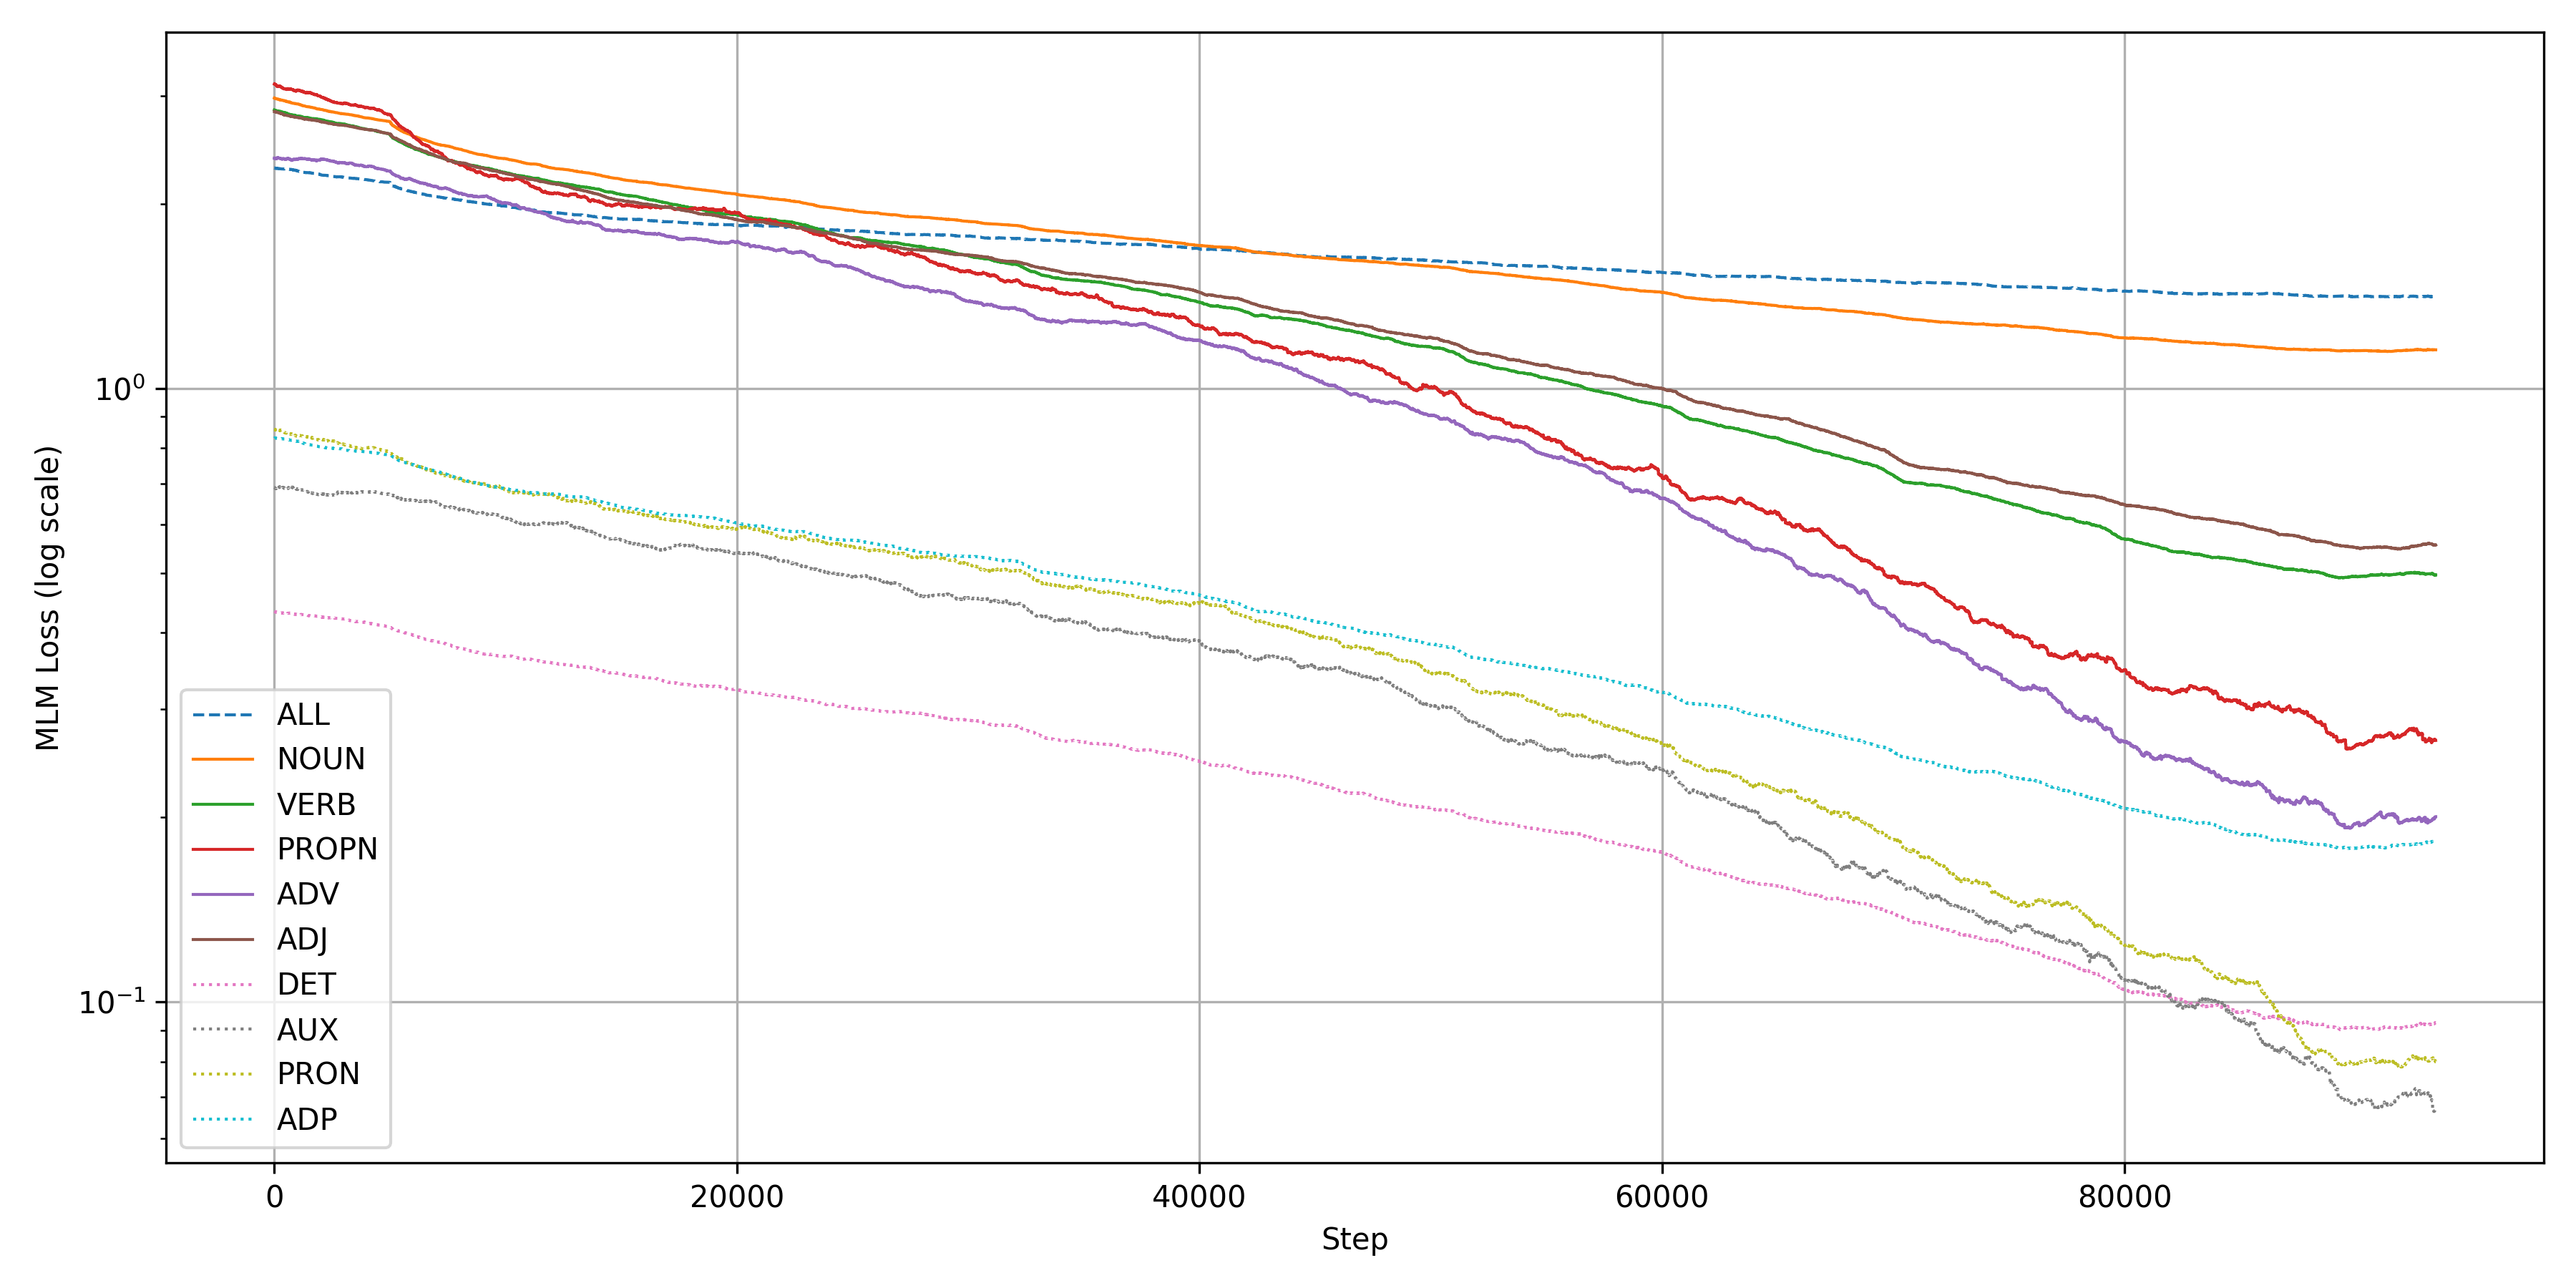
\includegraphics[width=1\textwidth]{Images/graph/mlm.png}
    \end{center}
\end{figure}

\begin{figure}[h]
    \caption{\acrshort{itc} loss curves for different \acrshort{pos} masking strategies (log scale).}
    \label{fig:itc_loss_pretrain}
    \begin{center}
        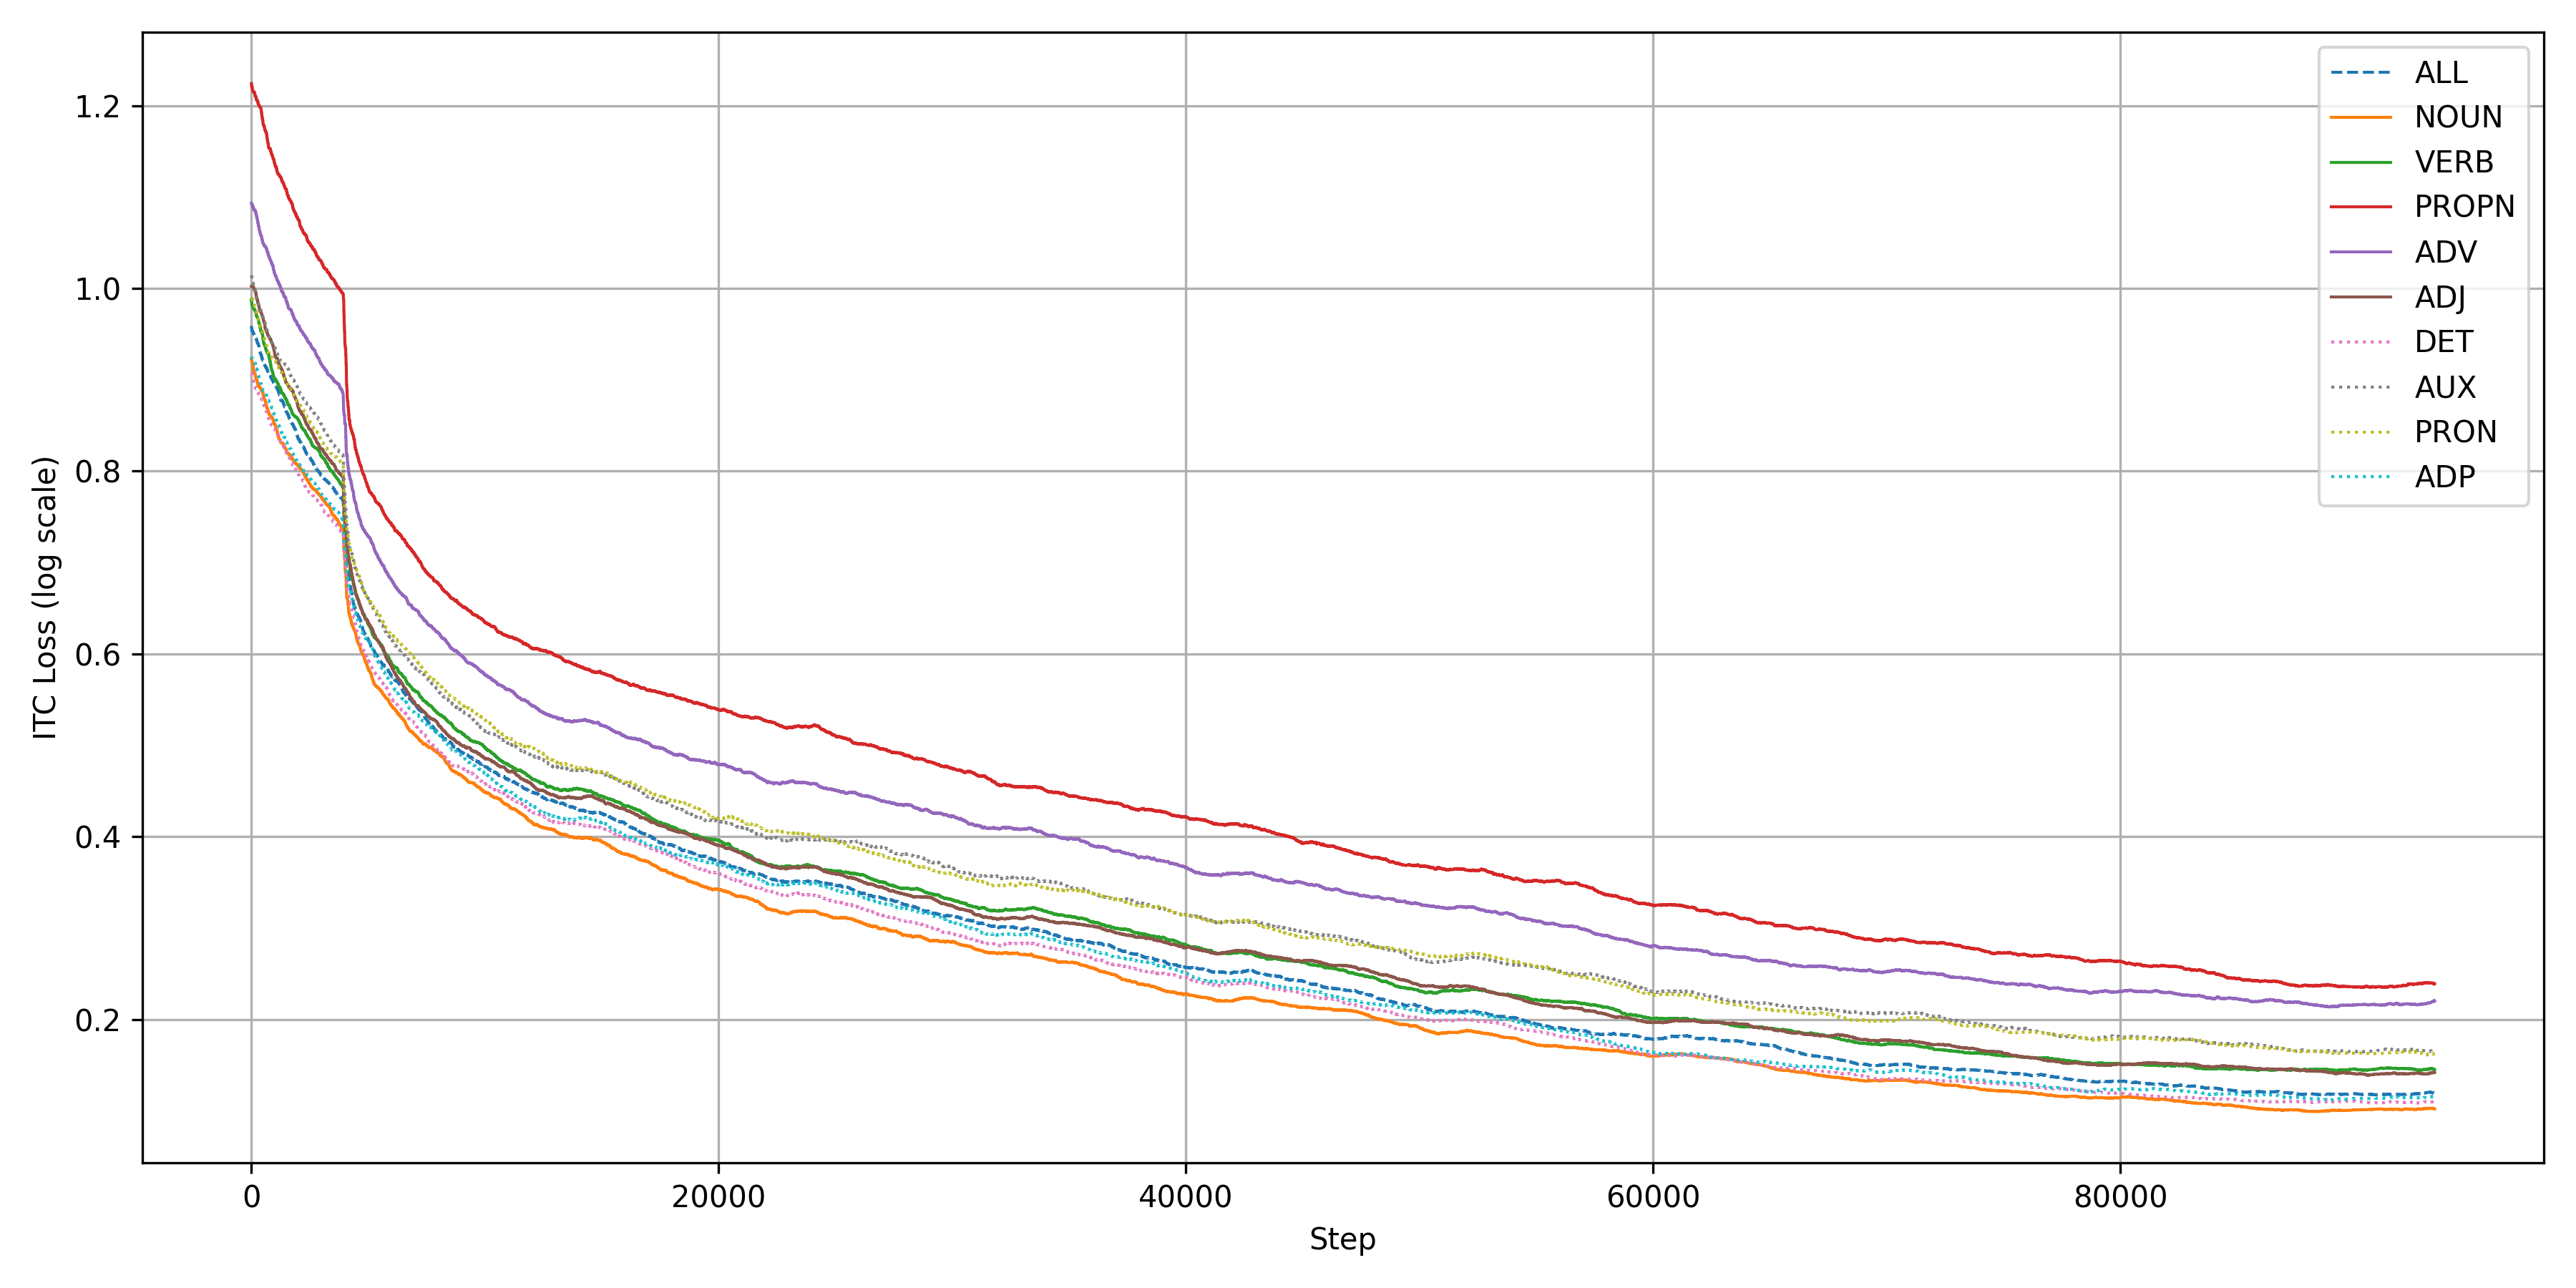
\includegraphics[width=1\textwidth]{Images/graph/itc.png}
    \end{center}
\end{figure}

\begin{figure}[h]
    \caption{\acrshort{itm} loss curves for different \acrshort{pos} masking strategies (log scale).}
    \label{fig:itm_loss_pretrain}
    \begin{center}
        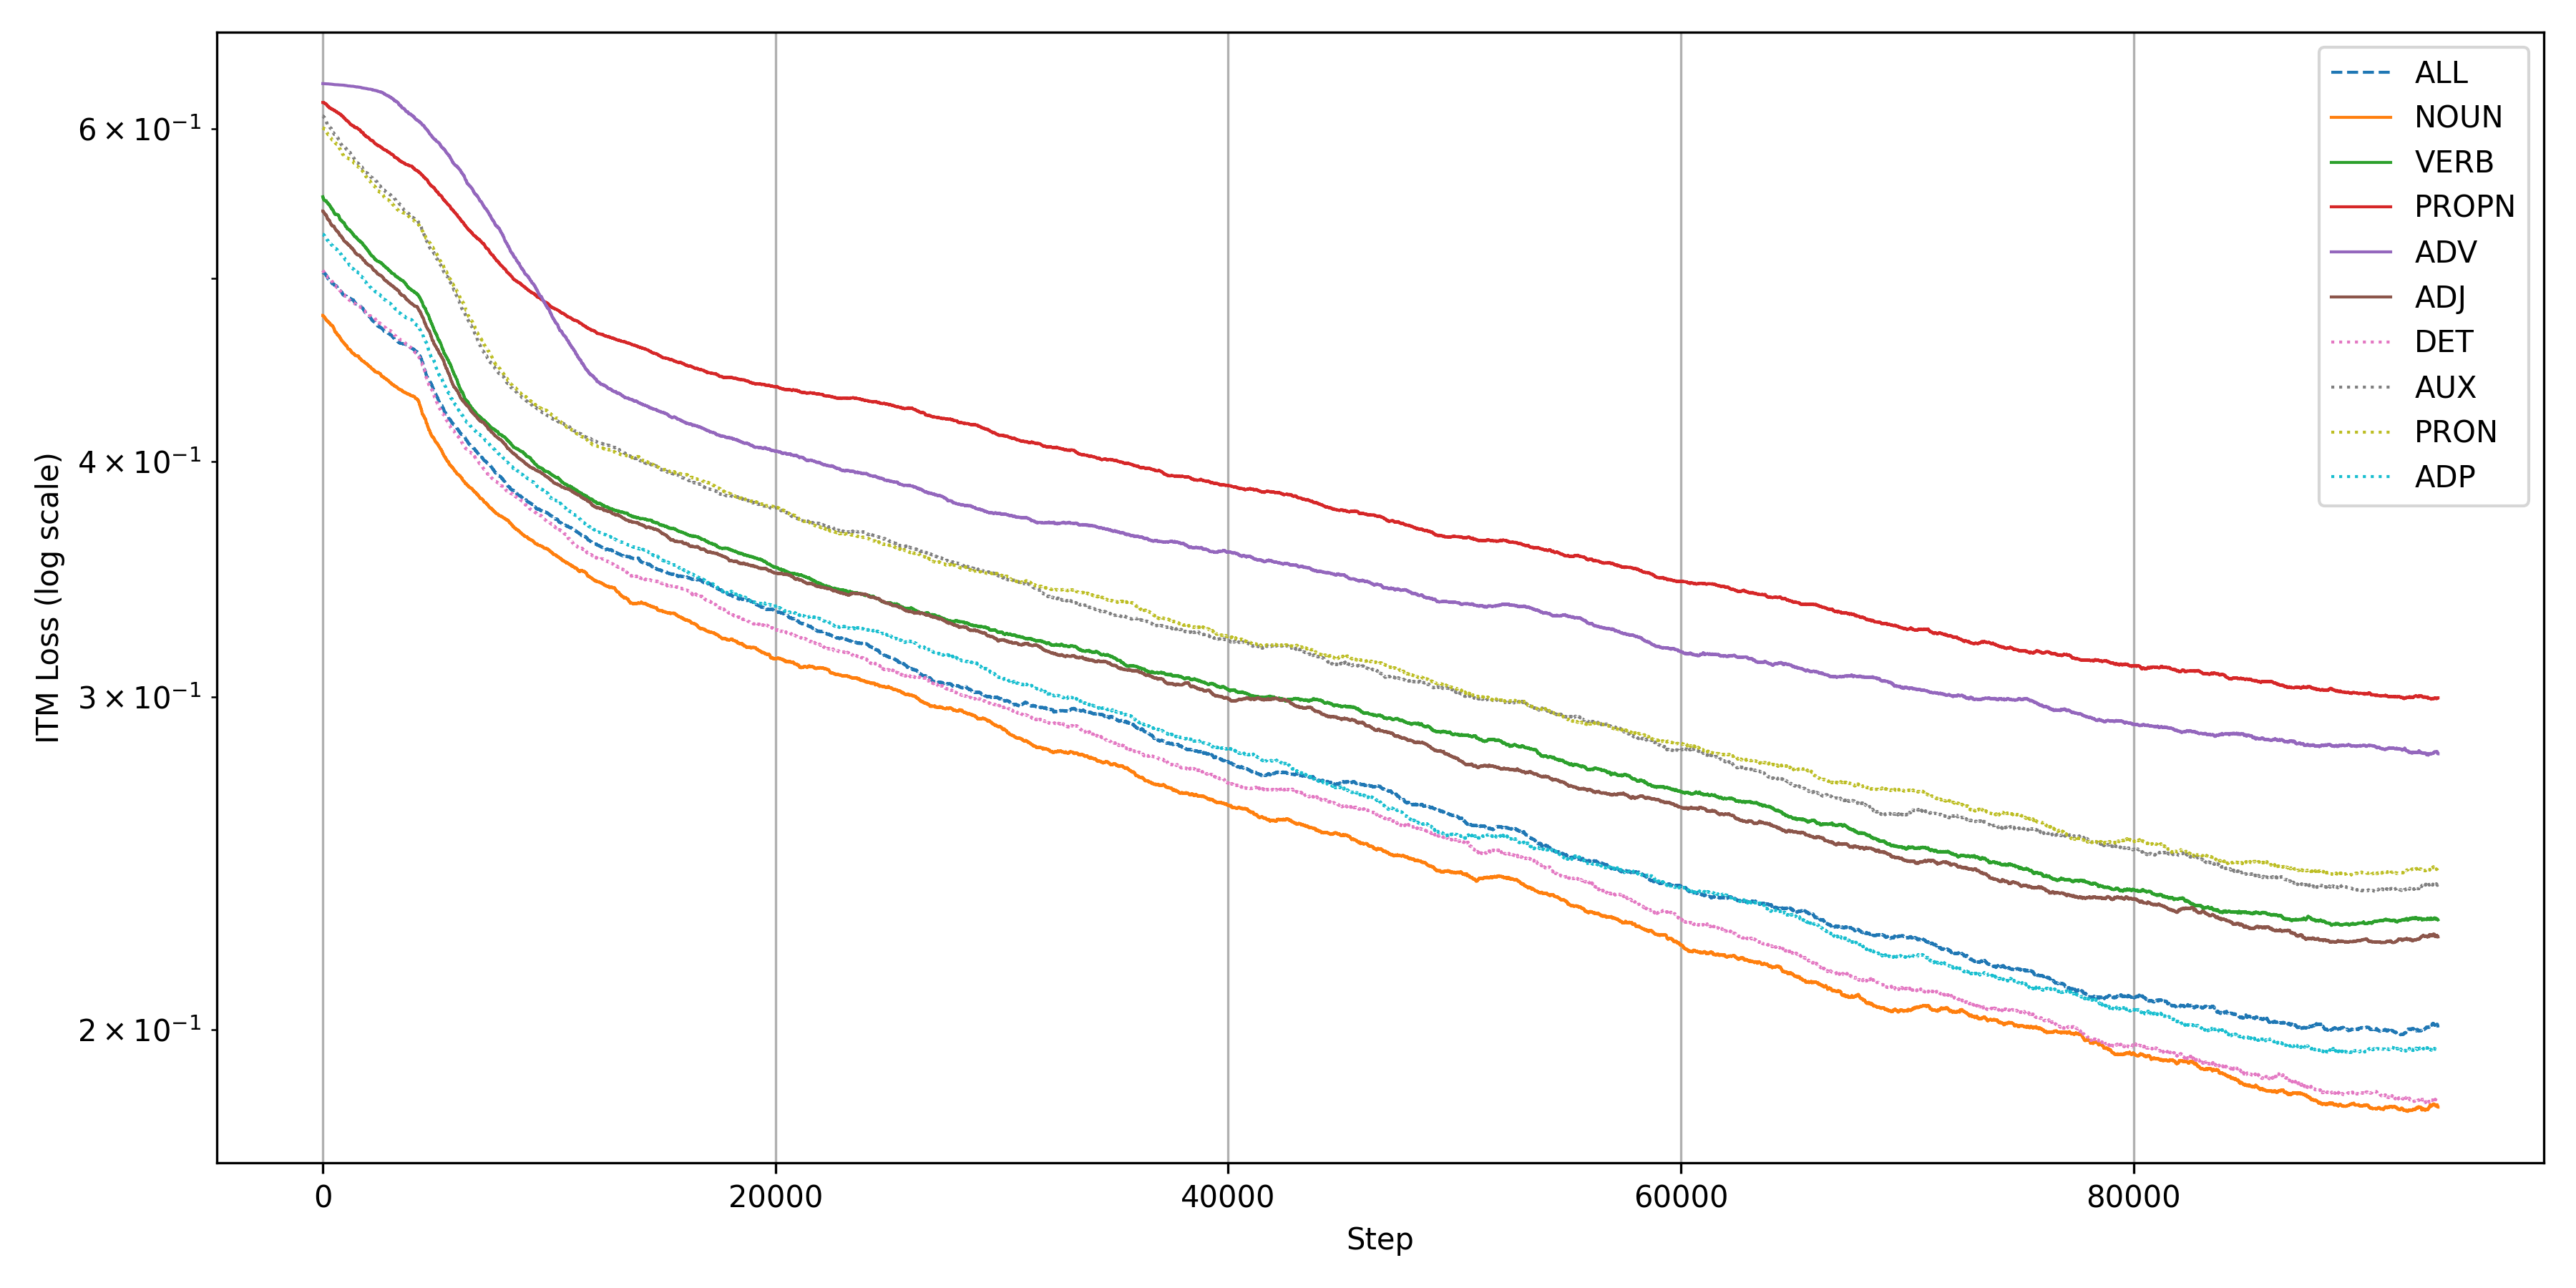
\includegraphics[width=1\textwidth]{Images/graph/itm.png}
    \end{center}
\end{figure}

\subsection{\acrshort{pos} Distribution in the Dataset}
To better understand the impact of POS masking, we analyzed the frequency distribution of each part-of-speech tag in the pre-training dataset.
As shown in Figure~\ref{fig:pos_count}, nouns are the most frequent category, followed by adpositions, determiners, and verbs.
In contrast, categories such as interjections, symbols, and punctuation appear infrequently and were not considered in the masking strategies due to their limited semantic contribution.

\begin{figure}[h]
    \caption{Histogram of POS tag frequencies in the training dataset (sorted by frequency).}
    \label{fig:pos_count}
    \begin{center}
        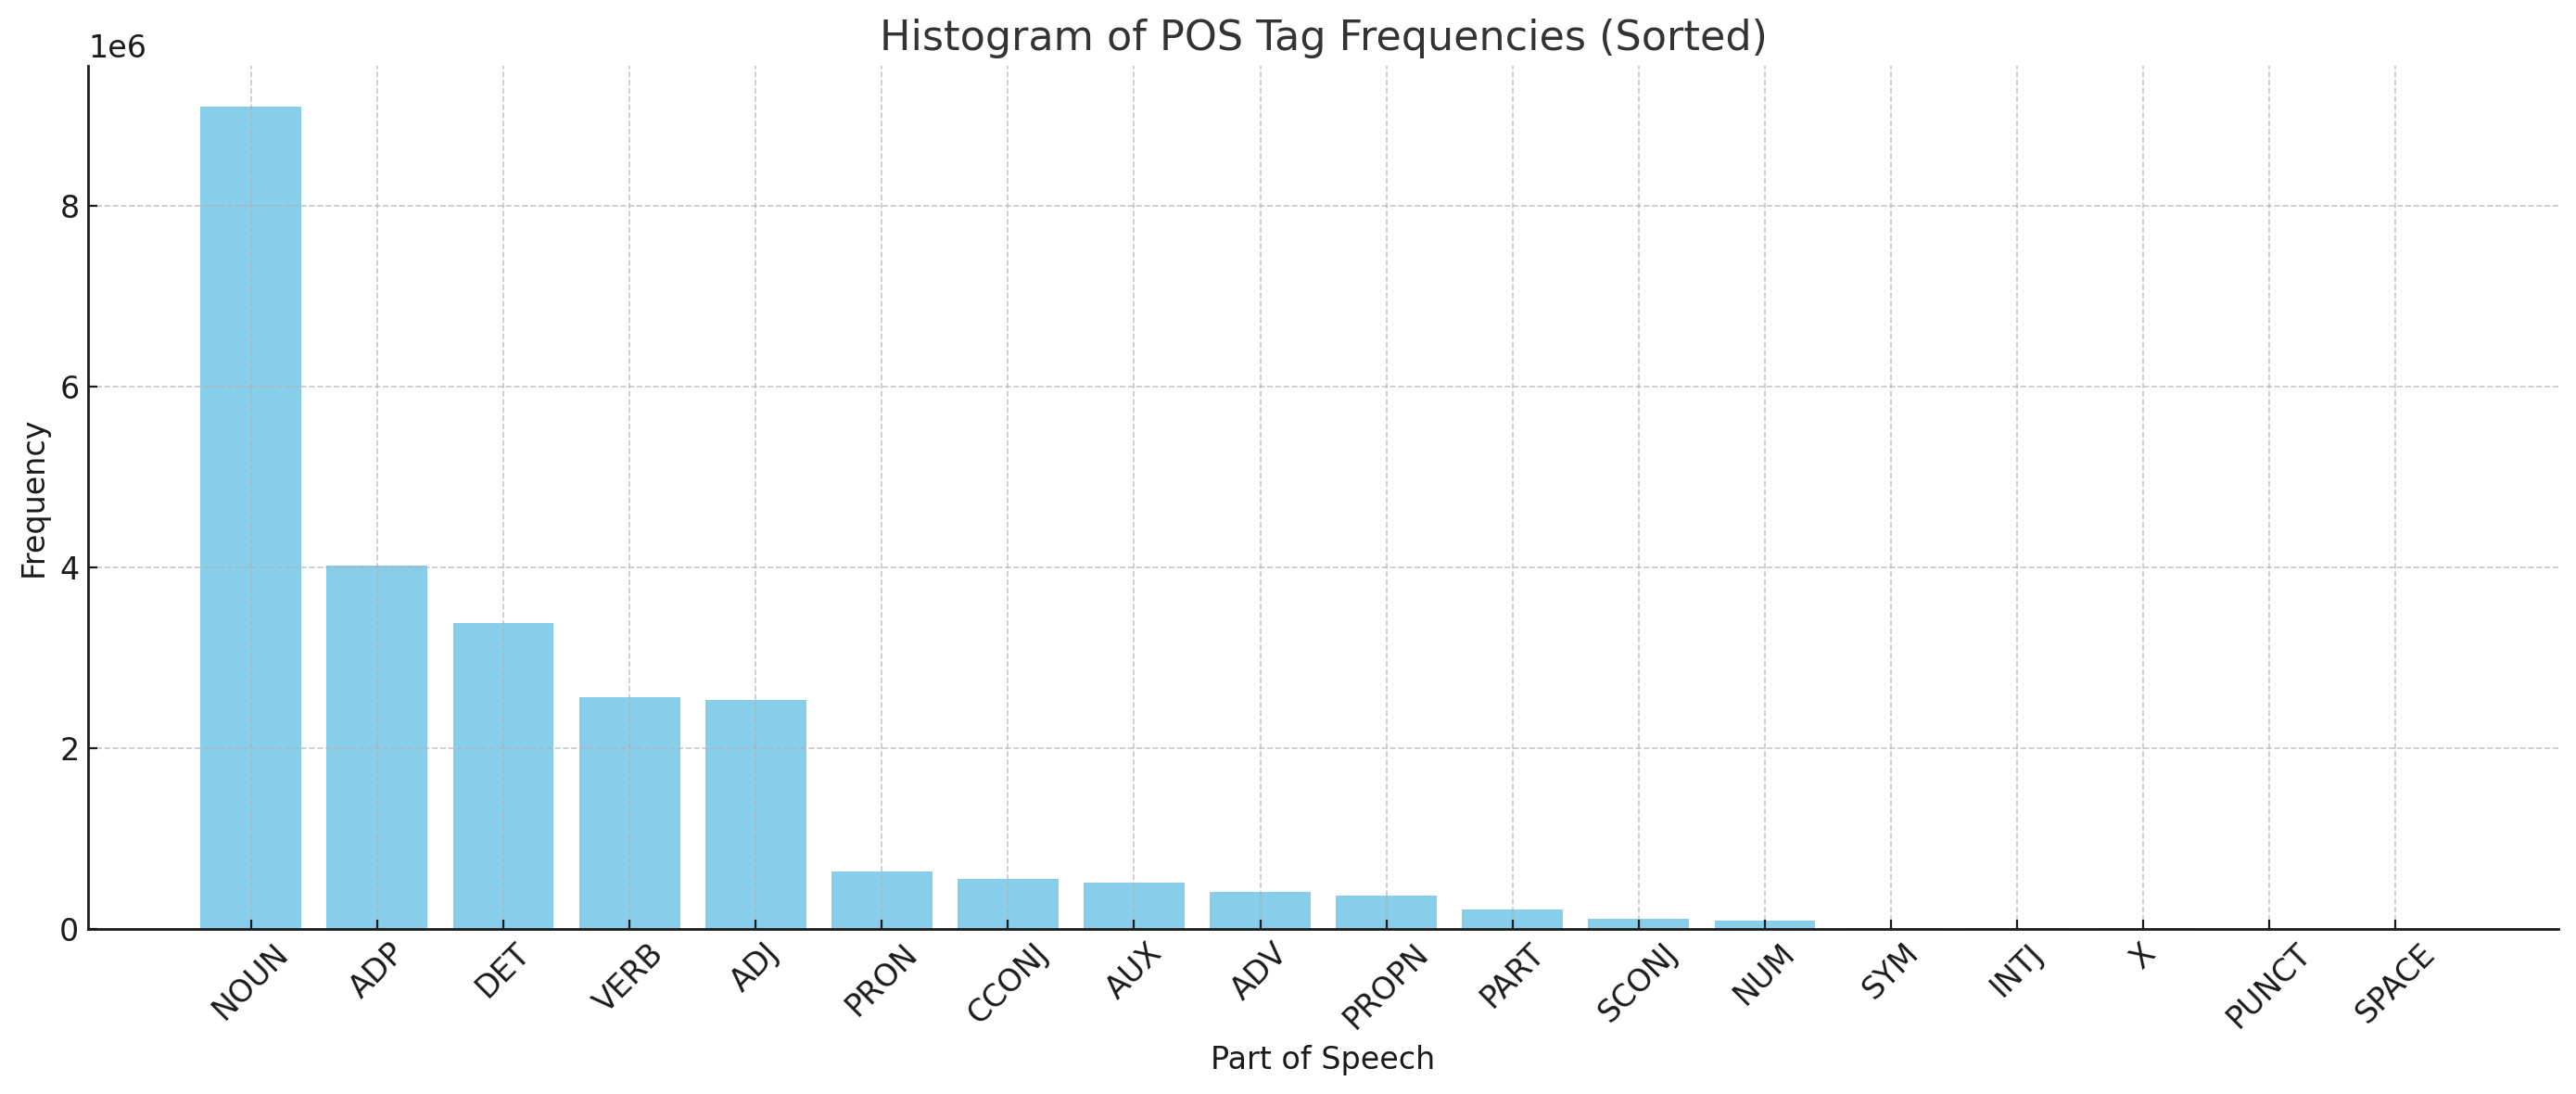
\includegraphics[width=1\textwidth]{Images/graph/pos_count.png}
    \end{center}
\end{figure}

\section{Image-Text Matching}
In this section, we evaluate the impact of \acrshort{pos} masking on image-text matching by reporting zero-shot classification accuracy on the VALSE benchmark.

\subsection{VALSE}
Table \ref{tab:valse} reports zero‐shot classification accuracy on the VALSE benchmark for each \acrshort{pos} masking strategy.  
The Random masking baseline yields a 60.20\%, serving as a reference point.  
Masking nouns further raises the average to 60.45\%, indicating that object words can be inferred from context in many cases.  
In contrast, masking verbs causes the average accuracy to drop to 58.66\%, with the largest degradation observed on the Relation and Action categories.  
Adjective masking attains an average of 59.24\%, showing that descriptive words contribute but are less critical than verbs.  
Masking adverbs and proper nouns leads to deeper declines, particularly on the Action and Coreference tasks, underscoring their role in temporal and referential understanding.  

These results highlight that the average accuracy (“Avg”) is the most indicative field for overall model competence, while the “Relation” and “Action” columns are especially informative for assessing the impact of verb and noun masking on fine‐grained relational and dynamic reasoning.

\begin{table}[]
    \centering
    \caption{VALSE benchmark for image-text matching result.}
    \label{tab:valse}
    \begin{adjustbox}{width=1\textwidth}
        \begin{tabular}{ll|c|c|ccc|c|cc|cc|c|c}
            \hline
            \multicolumn{2}{c|}{\multirow{3}{*}{\textbf{Masking Method}}} & \multicolumn{12}{c}{\textbf{VALSE}} \\
            & & Existence & Prularity & \multicolumn{3}{c|}{Counting} & Sp.Re \footnotemark & \multicolumn{2}{c|}{Action} & \multicolumn{2}{c|}{Coreference} & \multirow{2}{*}{Foil-it!} & \multirow{2}{*}{Avg} \\
            & & quantifiers & number & balanced & small number & adversarial & relations & replacement & actant swap & standard & clean & & \\
            \hline
            \multicolumn{2}{c|}{Random Masking} & 65.06 & 61.43 & \cellcolor{green}54.64 & 57.81 & 62.83 & \cellcolor{green}61.61 & 68.04 & 51.88 & 49.70 & 43.37 & 85.79 & 60.20 \\
            \hline
            \multirow{5}{*}{Non-function} & Noun & \cellcolor{green}67.63 & 62.60 & 52.59 & 54.64 & 64.39 & 59.84 & 68.15 & 48.87 & 51.31 & 49.21 & 85.69 & \cellcolor{green}60.45 \\
            & Verb & 60.37 & 60.50 & 54.83 & 56.30 & 61.52 & 57.68 & \cellcolor{green}68.24 & 48.62 & 51.30 & 42.40 & 83.45 & 58.66 \\
            & Adj & 60.85 & 60.55 & 54.00 & 56.84 & \cellcolor{green}67.01 & 57.68 & 65.68 & 50.92 & 50.34 & 44.74 & 83.01 & 59.24 \\
            & Adv & 62.56 & 58.74 & 53.08 & 57.32 & 59.92 & 58.10 & 65.74 & 49.11 & 49.04 & 41.30 & 84.28 & 58.11 \\
            & PropN & 61.51 & 59.23 & 52.49 & 56.25 & 61.26 & 55.86 & 64.31 & 50.85 & 50.36 & 43.03 & 82.62 & 57.98 \\
            \hline
            \multirow{4}{*}{Function} & Det & 60.14 & \cellcolor{green}63.33 & 53.47 & \cellcolor{green}57.86 & 65.40 & 59.06 & 66.67 & 50.43 & 50.09 & 38.99 & \cellcolor{green}87.94 & 59.40 \\
            & Aux & 56.73 & 60.60 & 51.76 & 57.32 & 60.59 & 56.48 & 65.04 & 50.65 & 49.33 & \cellcolor{green}51.39 & 84.62 & 58.59 \\
            & ProN & 56.05 & 61.33 & 50.39 & 54.88 & 58.87 & 58.93 & 64.36 & 48.05 & \cellcolor{green}53.23 & 50.48 & 83.40 & 58.18 \\
            & Adp & 66.27 & 61.23 & 53.52 & 57.03 & 66.04 & 58.28 & 67.73 & \cellcolor{green}52.14 & 50.05 & 46.13 & 86.38 & 60.44 \\
            \hline
        \end{tabular}
    \end{adjustbox}
\end{table}
\footnotetext{{Spacial Relation}}

\section{\Acrlong{vqa}}

\begin{table}[]
    \centering
    \label{tab:vqa}
    \caption{VQA2.0 test-dev benchmark result.}
    \begin{adjustbox}{width=0.6\textwidth}
        \begin{tabular}{ll|cccc}
            \hline
            \multicolumn{2}{c|}{\multirow{2}{*}{Masking Method}} & \multicolumn{4}{c}{VQA2.0 test dev} \\
            & & Yes/No & Number & Other & Overall \\
            \hline
            \multicolumn{2}{c|}{Random Masking} & 87.88 & 49.64 & 59.63 & 70.28 \\
            \hline
            \multirow{5}{*}{Non-function} & Noun & 87.84 & 49.49 & 60.03 & 70.29 \\
            & Verb & 87.17 & 48.39 & 58.43 & 69.13 \\
            & Adj & 86.69 & 48.86 & 58.64 & 69.09 \\
            & Adv & 83.10 & 43.83 & 52.49 & 64.12 \\
            & PropN & 85.07 & 46.38 & 56.60 & 67.71 \\
            \hline
            \multirow{4}{*}{Function} & Det & 87.35 & 49.49 & 57.68 & 68.98 \\
            & Aux & 85.25 & 46.59 & 56.24 & 67.09 \\
            & ProN & 84.13 & 46.29 & 56.15 & 66.55 \\
            & Adp & 87.07 & 48.82 & 58.07 & 68.96 \\
            \hline
        \end{tabular}
    \end{adjustbox}
\end{table}

\section{Masking Ratio}